\documentclass[a4paper, 11pt, fleqn]{article}

\usepackage{geometry}
\usepackage{geometry}
 \geometry{
 a4paper,
 total={210mm,297mm},
 left=23mm,
 right=23mm,
 top=30mm,
 bottom=30mm,
 }

\usepackage{amsmath}
\usepackage{amsfonts}
\usepackage{amsthm}

\usepackage[pdftex]{graphicx}
\usepackage{subcaption}

\usepackage{tikz}
\usetikzlibrary{arrows,shapes,backgrounds,through,shadows,snakes,patterns,mindmap}

\usepackage{fancyhdr}
\pagestyle{fancy}

%%   Document begins here   %%

\newcommand{\btheta}[0]{\boldsymbol{\theta}}
\begin{document}

 \title{Tensor Factorization for Relation Extraction}
\author{Marius Cobzarenco}
\maketitle

\section{Introduction}
% Matrix factorisation methods have been successfully applied to
% relation extraction tasks.
The problem of relation extraction can be formulated as a supervsied
learning problem where given a set $\mathbb{E}$ of entities/objects
and a set $\mathbb{P}$ of $n$-ary predicates the task is to learn new
predicates that may hold between the entities. A predicate (or
relation, both terms will be used interchangeably) is defined as a
boolean function $r:\mathbb{E}^n \rightarrow \{0, 1\}$.

\[examples of relations\]

For ease of comparison with previous work, we will focus on the case
of binary relations. However, all models discussed below are trivially
applicable to predicates of arbitrary arrity. Let us assume a training
set that consists of $ N_E \equiv \vert\mathbb{E}\vert$ entities, $N_R
\equiv \vert\mathbb{P}\vert$ relations and $N$ tuples
\begin{align}
X \equiv \{(i_n, j_n, k_n, r_n)\}_{n\in\overline{1..N}}
\end{align}
which are interpreted as asserting that relation $R_{k_n}$ either
holds ($r_n = 1$) or does not hold ($r_n = 0$) between entities
$e_{i_n}$ and $e_{j_n}$.
\begin{align}
R_{k_n}(e_{i_n}, e_{j_n}) &= r_n
\end{align}
The training tuples have the constraints that for $n\in{1..N}$ all
$(i_n, j_n, k_n)$ are distinct and
\begin{align}
1 \leq i_n \leq N_E, \quad 1 \leq j_n \leq N_E, \quad
1 \leq k_n \leq N_R,\quad r_n \in \left\{0, 1\right\}
\end{align}
Note that most natural language relations are not symmetric.

\begin{figure}[t]
\begin{center}
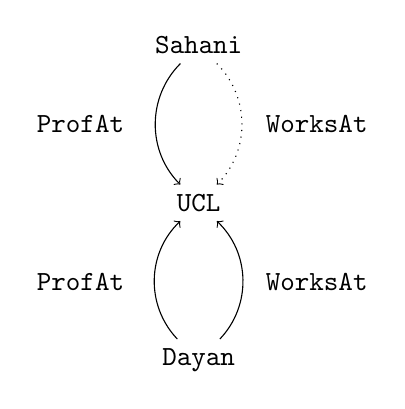
\begin{tikzpicture}[->]
\node(ucl) at (0,0) {\texttt{UCL}};
\node(pearson) at (0,2) {\texttt{Sahani}};
\node(dayan) at (0,-2) {\texttt{Dayan}};
\draw(pearson) to [bend right=45] (ucl);
\node at (-1.5,1) {\texttt{ProfAt}};
\draw[dotted](pearson) to [bend left=45] (ucl);
\node at (1.5,1) {\texttt{WorksAt}};
\draw(dayan) to [bend right=45] (ucl);
\node at (-1.5,-1) {\texttt{ProfAt}};
\draw(dayan) to [bend left=45] (ucl);
\node at (1.5,-1) {\texttt{WorksAt}};
\end{tikzpicture}
\end{center}
\end{figure}

\section{Tensor Decomposition}

\subsection{Log-Bilinear Model}
We propose modelling each entity $e_i$ as a real valued vector ${\bf
e}_i \in \mathbb{R}^D$ and each relation $R_k$ as a matrix ${\bf R}_k
\in \mathbb{R}^{D \times D}$. Given entities $e_i$ and $e_j$
the probability of a relation $R_k$ being true is modelled as
\begin{align}
  &p\left(R_k(e_i, e_j) = 1\vert \btheta\right) = \sigma\left({\bf
      e}'_i{\bf R}_k{\bf e}_j\right) \equiv \sigma\left({\bf
      e}'_i{\bf U}_k{\bf V}_k{\bf e}_j\right),
&\sigma(x) \equiv \left(1 + \exp(-x)\right)^{-1}
\end{align}
\noindent To make the embeddings interpretable and reguralize the
objective, ${\bf R}_k$ was constrained to be low rank ${\bf R}_k
\equiv {\bf U}_k{\bf V}_k$ for
some $ {\bf U}_k \in \mathbb{R}^{D
  \times \rho}$ and $ {\bf V}_k \in \mathbb{R}^{\rho \times D}$ with
$\rho \equiv \text{rank}({\bf R}_k) < D$. The parameters $\btheta$ are
the embeddings for entities and relations
\begin{align}
\btheta \equiv \{{\bf e}_i \vert i \in \overline{1..N_E}\} \cup
 \{{\bf U}_k, {\bf V}_k \vert k \in \overline{1..N_R}\}
\end{align}
An independent Gaussian prior with precision $\gamma$ was placed on
the coefficients of the embeddings
\begin{align}
  \forall i \in \overline{1..N_E}.\;\; {\bf e}_i \sim
  \mathcal{N}\left({\bf 0}, \sigma^2 \equiv \gamma^{-1}\right); \quad
  \forall k \in \overline{1..N_R}.\;\; {\bf U}_k[:], {\bf V}_k[:] \sim
  \mathcal{N}\left({\bf 0}, \sigma^2 \equiv \gamma^{-1}\right)
\end{align}
Given a dataset assumed assumed to be i.i.d., the posterior
distribution over $\btheta$ up to the normalisation constant is
\begin{align}
  \label{eqn:prob_dataset}
  p(\btheta\vert X) &\propto p(X\vert \btheta)p(\btheta) \nonumber \\
&= p\left(\left\{R_{k_n}(e_{i_n}, e_{j_n})=r_n\right\}_{n\in\overline{1..N}}\vert
    \btheta\right) p(\btheta)\nonumber \\
  &= \prod_{n=1}^{N}\left(1 - \sigma({\bf e}'_{i_n}{\bf R}_{k_n}{\bf
     e}_{j_n})\right)^{1 - r_n}\sigma({\bf e}'_{i_n}{\bf R}_{k_n}{\bf
      e}_{j_n})^{r_n} \prod_{i=1}^{N_E} (2\pi\sigma^2)^{-\frac{D}{2}}
    \exp\left(-\frac{{\bf e}_i'{\bf e}_i}{2\sigma^2}\right) \nonumber \\
&\times \prod_{k=1}^{N_R} (2\pi\sigma^2)^{-D\rho}
    \exp\left(-\frac{\text{Tr}\left({\bf U}_k'{\bf U}_k + {\bf V}_k{\bf V}_k'\right)}{2\sigma^2}\right)
\end{align}
This model can be fitted by finding the maximum a posteriori (MAP)
estimate $\btheta^* \equiv \operatorname{argmax} L(\btheta)$, with
$L(\btheta) \equiv \log p(X\vert \btheta)p(\btheta)$
\begin{align}
  \label{eqn:loglike}
  L(\btheta) &= \sum_{n=1}^{N}\left[ (1 - r_n) \log \left(1 -
    \sigma({\bf e}'_{i_n}{\bf R}_{k_n}{\bf e}_{j_n})\right) + r_n \log
  \sigma({\bf e}'_{i_n}{\bf R}_{k_n}{\bf e}_{j_n})\right] \nonumber \\
  &\quad - \frac{1}{2\sigma^2}\left[ \sum_{i=1}^{N_E} {\bf e}_i'{\bf e}_i
  +\sum_{k=1}^{N_R}
  \text{Tr}\left({\bf U}_k'{\bf U}_k + {\bf V}_k{\bf V}_k'\right)\right]
  - \frac{DN_E + 2D\rho N_R}{2}\log(2\pi\sigma^2)
\end{align}
The first term in the first summation in $L(\btheta)$ can be rewritten as
\begin{align}
(1 - r_n) \log \left(1 -
    \sigma({\bf e}'_{i_n}{\bf R}_{k_n}{\bf e}_{j_n})\right) =
  (r_n - 1)\left( {\bf e}'_{i_n}{\bf R}_{k_n}{\bf e}_{j_n} +
  \log(1 + \exp(-{\bf e}'_{i_n}{\bf R}_{k_n}{\bf e}_{j_n})) \right)
\end{align}
This helps with numerical stability when the sigmoid would otherwise
saturate. The function $log(1 + x)$ is often implemtened in numerical
packages as \texttt{log1p} such that it is accurate for small $x$
where $1 + x = 1$ in floating point arithmetic. $L$'s partial
derivatives w.r.t. $\btheta$ can be computed as
\begin{align}
  \label{eqn:objective}
  \frac{\partial L}{\partial {\bf U}_k} &=
  \sum_{n=1}^{N}\delta_{k,k_n}\left[(r_n - 1)\sigma({\bf
      e}'_{i_n}{\bf R}_{k}{\bf e}_{j_n}) + r_n \left( 1 - \sigma({\bf
        e}'_{i_n}{\bf R}_{k}{\bf e}_{j_n}) \right)\right]
  {\bf e}_{i_n}{\bf e}'_{j_n}{\bf V}'_k- \frac{1}{\sigma^{2}}{\bf U}_k \\
  \frac{\partial L}{\partial {\bf V}_k} &=
  \sum_{n=1}^{N}\delta_{k,k_n}\left[(r_n - 1)\sigma({\bf
      e}'_{i_n}{\bf R}_{k}{\bf e}_{j_n}) + r_n \left( 1 - \sigma({\bf
        e}'_{i_n}{\bf R}_{k}{\bf e}_{j_n}) \right)\right]
  {\bf U}'_k{\bf e}_{i_n}{\bf e}'_{j_n} - \frac{1}{\sigma^{2}}{\bf V}_k \\
  \frac{\partial L}{\partial {\bf e}_i} &=
  \sum_{n=1}^{N}\left[(r_n - 1)\sigma({\bf
      e}'_{i_n}{\bf R}_{k_n}{\bf e}_{j_n}) + r_n \left( 1 - \sigma({\bf
        e}'_{i_n}{\bf R}_{k_n}{\bf e}_{j_n}) \right)\right] \left( \delta_{i,i_n}{\bf R}_{k_n}
    {\bf e}_{j_n} + \delta_{i,j_n}{\bf R}'_{k_n} {\bf
      e}_{i_n}\right)\nonumber \\
  &\qquad - \frac{1}{\sigma^2} {\bf e}_i
\end{align}
\noindent One problem with this simple model is that in practice the
training set would come from a knowledge base which mostly if not
completely contains positive facts. This results in a highly
unbalanced dataset where most $r_k = 1$ and the model will just learn
to output 1. One simple fix is to generate negative examples by
sampling a random relation and two entities for each positive training
example. The assumption is that relations are highly sparse and only
hold for a few combinations of entities.
\subsection{Bayesian Personalised Ranking}

The challenge of learning only from positive feedback is very similar
to collaborative filtering with implicit feedback. For example, when
recommending products based only on the shopping history of a
customer, there's no information in the training set about the
products that customers do not like. Similarly, a knowledge base only
contains entity pairs that a relation ``likes''. A principled to
approach learning only from positive examples is to use a ranking
objective. Instead of explicitly modelling the probability of a
relation being true, the new objective would learn an ordering of
entity pairs for each relation.
\begin{align}
  p\left( (e_i, e_j) >_{k} (e_m, e_n) \vert \btheta\right) &\equiv
  p\left( R_k(e_i, e_j) > R_k(e_m, e_n) \vert \btheta\right) \nonumber \\
  &= \sigma\left( {\bf e}'_i{\bf R}_k{\bf e}_j -
    {\bf e}'_m{\bf R}_k{\bf e}_n\right )
\end{align}
\noindent The \emph{Bayesian Personalised Ranking} (BPR) objective was first
proposed for collaborative filtering datasets with implicit feedback
\cite{rendle2009bpr}. It had been used in the context of relation
extraction in \cite{riedel13relation} where it ranked the output of a
matrix factorisation algorithm over entity pairs and relations.
\noindent Given a training set, the BPR objective enforces that
observed relations are more likely than the unobserved ones.
\begin{align}
  \bar{X} &\equiv \left\{(k,i,j,m,n)\vert R_k(e_i, e_j) \in X \wedge R_k(e_m, e_n) \notin X \right\} \\
  p(X\vert\btheta) &= \prod_{k=1}^{N_R}p(>_k\vert \btheta) =
  \prod_{\in\bar{X}} p\left( (e_i, e_j) >_{k} (e_m,
    e_n)\vert \btheta \right) \\
  \text{BPR}(\btheta) &\equiv \log \left( p(X\vert\btheta) p(\btheta)
  \right)
  \nonumber \\
  &= \sum_{\in\bar{X}} \log \sigma\left( {\bf e}'_i{\bf R}_k{\bf e}_j
    - {\bf e}'_m{\bf R}_k{\bf e}_n\right ) + \log p(\btheta) \nonumber
  \\
  \label{eqn:bpr_obj}
  &\propto \sum_{\in\bar{X}} \log \sigma\left( {\bf e}'_i{\bf R}_k{\bf
      e}_j - {\bf e}'_m{\bf R}_k{\bf e}_n\right ) +
  \frac{1}{2\sigma^2}\left[ \sum_{i=1}^{N_E} {\bf e}_i'{\bf e}_i
    +\sum_{k=1}^{N_R} \text{Tr}\left({\bf U}_k'{\bf U}_k + {\bf
        V}_k{\bf V}_k'\right)\right]
\end{align}
The partial derivatives of $\text{BPR}(\btheta)$ with respect to the
entity and relation embeddings can be computed as
\begin{align}
  \label{eqn:bpr_grad}
  \frac{\partial\text{BPR}}{\partial {\bf U}_l} &= \sum_{\in
    \bar{X}}\delta_{k,l}\sigma\left( {\bf e}'_i{\bf R}_k{\bf e}_j -
    {\bf e}'_m{\bf R}_k{\bf e}_n\right ) \left( {\bf e}_{m}{\bf
      e}'_{n}{\bf V}'_k-{\bf e}_{i}{\bf e}'_{j}{\bf V}'_k\right )
  - \gamma{\bf U}_l \\
  \frac{\partial\text{BPR}}{\partial {\bf V}_l} &= \sum_{\in
    \bar{X}}\delta_{k,l}\sigma\left( {\bf e}'_i{\bf R}_k{\bf e}_j -
    {\bf e}'_m{\bf R}_k{\bf e}_n\right ) \left( {\bf U}'_k{\bf
      e}_{m}{\bf e}'_{n} - {\bf U}'_k{\bf e}_{i}{\bf
      e}'_{j} \right) - \gamma{\bf V}_l \\
  \frac{\partial \text{BPR}}{\partial {\bf e}_l} &= \sum_{\in
    \bar{X}}\sigma\left( {\bf e}'_i{\bf R}_k{\bf e}_j - {\bf e}'_m{\bf
      R}_k{\bf e}_n\right ) \left( {\bf R}_{k}(\delta_{l,m} {\bf
      e}_{n} - \delta_{l,i}{\bf e}_{j}) + {\bf R}'_{k}(
    \delta_{l,n} {\bf e}_{m} - \delta_{l,j}{\bf e}_{i})
  \right) - \gamma {\bf e}_l
\end{align}
\noindent We follow \cite{rendle2009bpr} and replace the objective
above with a stochastic version. We propose optimising the BPR
objective using Nesterov's Accelerated Gradient (NAG) method.

\bibliographystyle{plain}
\bibliography{refs/refs.bib}

\end{document}
